

%\documentclass{scrippsthesis}
\documentclass[a4paper,11pt,twoside]{UUthesis}
%\usepackage[pass]{geometry}
%%% HEADER INFORMATION %%%

\title{Network Traffic Simulator:  \\ Designing an Extensible Traffic Management System Using Python}
\author{Julia Ruiter}
\advisor{Yannis Velegrakis}
\reader{Ioana Hulpis}
\department{Department of Natural Sciences}

%%% Including new commands and packages.

% Allows for auto formatting of theorems,
% definitions etc.
\usepackage{amsthm}
\usepackage{graphics,graphicx}
\usepackage{tikz}
\usepackage{verbatimbox}
\usepackage{textgreek}
\usepackage[toc,page]{appendix}
\usepackage{float}
\usepackage{amsmath}
\usepackage{hyperref}

\usepackage{alltt}   % alternate method for pretty code -- SUPPORTS BOLD
\renewcommand{\ttdefault}{txtt}

% \usepackage{listings}   % display python code nicely
% \lstset{                 % allow verbatim to auto-line-break
% basicstyle=\small\ttfamily,
% columns=flexible,
% breaklines=true
% }
% \lstset{language=Python}



\usepackage{etoolbox}   % prevent bibliographies from splitting on pagebreak
\apptocmd{\thebibliography}{\interlinepenalty 10000\relax}{}{}



\newtheorem{thm}{Theorem}[chapter]
\newtheorem{lem}[thm]{Lemma}
\newtheorem{prop}[thm]{Proposition}
\newtheorem{cor}[thm]{Corollary}

\theoremstyle{definition}
\newtheorem{defn}[thm]{Definition}
\newtheorem{ex}[thm]{Example}

\theoremstyle{remark}
\newtheorem*{rmk}{Remark}
\newtheorem*{notn}{Notation}
\newtheorem*{pf}{Proof}

% Add any new commands here.
\newcommand{\Q}{\mathbb{Q}}
\newcommand{\Z}{\mathbb{Z}}
\newcommand{\F}{\mathbb{F}}
\newcommand{\R}{\mathbb{R}}
\newcommand{\NN}{\mathbb{N}}

%file path for images


%%%  END HEADER %%%

\begin{document}
%\begin{comment}

\frontmatter

\maketitle % Title page


%%%% ABSTRACT.
\begin{abstract} 
This paper documents the creation of an extensible traffic management system that can be used to simulate various graph problems from congestion in city traffic, to distribution and shipping logistics, to internet traffic.  The Network Traffic Simulator design process and motivation have been fully described, and the paper is complete with a tutorial on how to use the software to solve your own network traffic problems.
\end{abstract}

%%% ACKNOWLEDGEMENTS.
\begin{acknowledgments}
I'm extremely grateful for my partner, Warren Fletcher, for all the support he has provided me (both professionally and emotionally) in the duration of both thesis and this entire master's program. He has given invaluable guidance in writing and designing a proper/professional piece of software, and has patiently helped fill in the gaps in my computer science knowledge, pointing me in the right direction for data structure and algorithm usage.  This project would not be possible without the many design debates and ensuing suggestions from him.
\end{acknowledgments}

%%% CONTENTS, FIGURES, TABLES
\tableofcontents
\listoffigures
%\listoftables

%%% End of the front matter.

%% MAIN MATTER - INCLUDE THE CHAPTERS.
\mainmatter

% CHAPTERS %
\chapter{Introduction}
\chapter{Existing Traffic Simulation Models}
\label{Related}

\par The majority of popular open-source network modeling software focus explicitly on single network types.  SUMO is used for detailed urban traffic simulations for physical 
(like SUMO, of NS2) focus specifically on 
\chapter{Design Motivations}
\label{Motivations}

\par The goal of this project was to design and code a general solution to the traffic modeling problem. After all--if one can prove that the generalized solution works, then any special case should, too, thus satisfying the aim to create an extensible and multi-use simulation model.  \\

\par   To prove so requires combining graph theory, combinatorics, and data structures. However, computers require a bit more work to conform to the natural mathematics of graph theory as they force discreteness.  This meant that special considerations had to be made to emulate the continuous real-world systems it may be required to simulate.  With real-world precision and accuracy as the utmost goal, the system was designed with the following criteria: \\


\section{Network Structure:  how should the network be stored in memory?}
\par Nodes are connection points for several edges, like road intersections, cellular towers, etc.  By utilizing graph data structures, one can also take advantage of the numerous existing path-finding algorithms and easily keep track of connected pair of nodes (and their directionality). \\

\par The advantages of designing a directed graph model rather than undirected are obvious:  car lanes force traffic in a particular direction, and packets of information cannot necessarily be transmitted in both directions (especially if there are intermediary steps, like encryption, that are not reversible). \\

Further continuing with intuitive design decision, it followed that the network needed to be directional, and that multiple parallel edges between a pair of nodes should be allowed.  Directionality's reason is easy to sport:   \\  


\par Directionality has another advantage in that it allows for multiple parallel edges.  This has the added benefit of intuitively and adaptably being able  to increase (or restrict) edge capacity, serving as another parameter the user can tune to mimic real-world constraints.  This ensures that this traffic simulator has the flexibility to model microscopic and macroscopic traffic trends \cite{LWB18}.  Using normal commuting traffic as an example, a user can test whether or not adding another lane to a freeway (or adding lane accessible to cars only of a certain type) would ease congestion as they are able to view metrics and positionality per timestamp of the entire system (macroscopic), the set of edges between two nodes or each individual node (mesoscopic), and the individual cars on those roads themselves (microscopic) \cite{LWB18}. \\


\par Though some traffic simulations in existence use adjacency matrices to define neighbouring nodes \cite{GPK02}, this is not a scalable, nor desirable, solution .  While adjacency matrices are intuitive for humans to read and understand, since most networks are fairly sparse they end up storing a lot of NULL values and require n! complexity to process those NULLs.  While little heed is paid to memory conservation in the rest of this simulation's design process, the idea of holding space for nonexistent edges did not seem like a very good idea.  Instead, it makes sense to think more about the interactions of node-edge pairs via their object pointers.  Adjacency matrices acknowledge that an edge is defined by its originating and terminal nodes, but fails to demonstrate how a node is only interesting because of the set of inbound and outbound edges it connects.  To capture both of these ideas, dictionary mappings were utilized to identify and link nodes to edges and edges to nodes, allowing either or both interactions to be utilized, depending whichever one was more intuitive for the particular action being done at any point in the simulation process.\\

\begin{figure}[H]
    \centering
	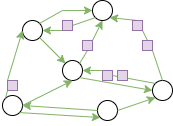
\includegraphics[width=0.5\textwidth]{tex files/Figures/generic_network.png}
	\caption[Random directional network]{Proposed structure:  random directional network with objects on it, with one edge per possible object-carrying "lane" (non-redundant)}
	\label{fig:generic_network}
\end{figure}

% TODO:  closeup image of path/when nodes used/when edges used

\section{How does the traffic network change state, processing car movement?}

\par A methodical process is needed to execute all the actions that can take place on each tick of the simulator (tick being the function that executes said changes for each incremental timestamp in the simulation runtime).  Once all available or possible actions have been made for that tick, the simulation is considered to be in a new state, and that information about that state is returned to the user. \\

\par The network object consists of nodes and edges, so it makes sense to break down the action queue to these levels as well.  However, you can't just arbitrarily run all nodes and edges as there is an inherent order and hierarchy to them.  As edges are defined by their start and end nodes, it makes sense to have edge tick processes as a dependent of node tick processes.  Furthermore, because nodes are capable of having multiple inbound and outbound edges, it is essential to process a particular node's edge ticks together to ensure as smooth and realistic of a movement between edges as possible. \\

\par To ensure that each component of a network is only processed once, on each tick, the network tick function iterates through all nodes listed in the network's node dictionary.  Each node, in turn, processes each outbound edge in its adjacent outbound edges dictionary.  The network tick and its subsequent node and edge ticks will be performed as many times as necessary until the cars run out of energy (more on that later in the \textbf{Movement} section) \textit{or} no more advances can be made with the current remaining energy potentials, and report out the number of loops needed to do so and the total percent of potential energy used.  These values can be used as a proxy for network congestion, though more as a benchmark between ticks or simulations than as an absolute value of ability. \\

\par To ensure that no node nor edge is favored (ei: always has their candidate cars move before any other node or edge's), the order in which these items are iterated is shuffled with each pass.  While this helps immensely with simulation accuracy, the random nature is what prevents the output numbers from being a reliable and accurate metric of network (in)action. 


\section{Where should car location be stored?}

\par A traffic simulation is not very insightful without considering the things which themselves cause traffic--Who, or what, keeps track of where the "cars" are?  Though innocuous, the question leads to some philosophical fancies that need to be addressed before determining who (or what) is in charge of your position. \\

\par If you're driving home at midnight, you might choose to take a faster route or a more scenic route, you might pull over to look at the citylights or take a pause because you're feeling sleepy, or you might drive a bit over the speed limit up because there's not likely to be any cops on the road at this hour of night.  It feels like you own the road and you have full control over where you are right here right now.  \\

\par But what if you (are trying to) drive home 5 o'clock Friday in the thick of traffic?  Yes, you \textit{chose} to take a particular route home, but now you're stuck in bumper-to-bumper traffic and can't move forward til the car in front of you decides to (or can at all).  While you may be in control of your car, you don't have full control over your ability to move, and thus over your position.  This leads to the inevitable conclusion that a simulation will be most accurate if the network controls the cars rather than letting the cars control themselves, meaning that current position must be stored on the objects over which the cars are moving:  the edges.


\section{Discrete versus continuous systems:  how is position represented?}

\par Since edges store car locations and move them along a particular distance each unit of time, it's tempting to think of positions in terms of capacity.  If an edge is 10 units long and cars travel 2 units per time, there are 5 positions a car can be, so a car's position can be stored as its index in the capacity queue.  This makes movements easy to simulate and requires a minimal, fixed storage space no matter the amount of cars on the network.  So this is that design choice, right? \\

\par ...well, not quite.  Sure, the example above is easy to quantify, but breaks down when situations arise that obstruct predictable movement, ranging from traffic jams to even just switching to an edge with a different speed limit.  If a car is unable to move its full potential, it's then unable to move into the next discrete state.  So where does it go? And where do any cars after it go? \\

\par The problem with defining position by the distance a car can go at it's maximum speed is that there's a lot of unaccounted distance.  If a car is going 10 m/min, then the position would be defined as 10 meters later (if the unit time distance of the simulation were in minutes)--in a road stretch of 60 meters, there would be 6 possible positions.  \\

\begin{figure}[H]
    \centering
	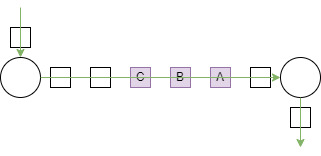
\includegraphics[width=0.75\linewidth]{tex files/Figures/BasicDiscrete_Before.png}
	\caption[Discrete positions: example]{Example discrete system with 6 slots, 3 of which currently occupied}
	\label{fig:BasicDiscrete_before}
\end{figure}


\par Now let's say that the car (car A) has reached the end of the road segment and is trying to turn onto a crossroad, but the crossroad is completely full.  Car A must stop at the end of the road segment and wait for an opening.  The car behind (car B), meanwhile, is still driving 10 m/min but must stop before crashing into the halted car in front, but any cars behind it are still capable of moving fully into the next position in the queue.  Where is Car B?  It cannot be in the final position (as Car A is still occupying it), and the penultimate position is now taken up by Car C which was one position behind Car B.\\

\begin{figure}[H]
    \centering
	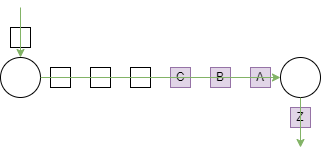
\includegraphics[width=0.75\linewidth]{tex files/Figures/BasicDiscrete.png}
	\caption[Discrete positions: blockade]{No obstructions yet:  all cars have proceeded one slot forward}
	\label{fig:BasicDiscrete}
\end{figure}


\par Faced with this situation in a discrete system, we must compromise on simulation accuracy:  either you allow cars to pile up on positions (defeating the purpose of a queue \textit{and} unrealistically depicting car location), or you prevent cars from moving at all (artificially causing traffic on the current edge when there is, in fact, room to move.  This cascades onto other connected edges and may stall the whole simulation).  While option one doesn't seem too terrible, it runs the risk of allowing cars to "jump" over halted cars; if car C's destination is the location car A is stuck, then when car C piles onto the position two timestamps later, it registers as completing its journey despite that being impossible in a real-world scenario.  \\

\begin{figure}[H]
    \centering
	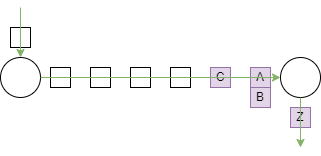
\includegraphics[width=0.75\linewidth]{tex files/Figures/BasicDiscrete_Overlap.png}
	\caption[Discrete positions: multiple cars at one location]{Car A is stuck, car B and C advance, causing car B to share a spot with car A}
	\label{fig:BasicDiscrete_overlap}
	
	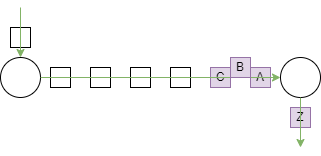
\includegraphics[width=0.75\linewidth]{tex files/Figures/BasicDiscrete_between.png}
	\caption[Discrete positions: non-fixed locations]{Car A is stuck, car B advances to an in-between stage, Car C advances one slot forward}
	\label{fig:BasicDiscrete_between}
\end{figure}

\par It is clear that some other solution is needed if a realistic simulation is to be created.  And that solution is simple:  switch to floating point positions.  By mapping cars to their exact position from 0 to maximum edge length, the user can be explicit about how long each car is and how close the cars are allowed to be to each other, all the while ensuring accuracy in car behavior by preventing skipping.  While this adds additional complexity to movement calculations, the resulting affinity for precision solves any practical or logical issues that a discrete system would incur.


\section{On Paths, Origins, and Destinations}

\par "How do I get from Point A to Point B?" and what even constitutes a "point"?  Path-finding algorithms typically find the fastest/shortest/"best" route between any 2 given nodes, which would imply that nodes are the points. This intuitively makes sense and works great for simulation paths with bounded, real-world constraints.  Take (a very simplified example of) email communication:  emails will always start at one machine (node), travel to a server (node), and perhaps be passed onto another server for the receiver to view (node); there might be more or less steps between each landmark, but the only place a message can originate is at one of the endpoints.  \\

\par However, cars do not spawn in the middle of a four-way intersection, nor does it make sense to create a network model where every possible parallel parking spot is a separate node in a network.  For one, someone could do a terrible parking job and take up two spots, therefore creating some new start or end node somewhere between the existing spots.  But the more pressing issue with breaking a road into n continuous, sequential, connected segments is the same sort of unwanted inefficiency as the adjacency matrices proposed earlier:  there's a lot space and computation wasted on pairs that generally provide no function to the simulation. \\

\par This led me to turn the usual graph structure on its head, and instead allow cars to enter and leave the network from the edges themselves.  To make this work for traditional node-to-node paths, the car placement mechanism has been written in such a way that if no specific edge location has been specified for a start and end point, a path is selected based on those nodes and the "car" is placed at position 0 along the first edge (and finishes its journey at the maximum length of the final edge, or effectively at the terminal node). \\

\par Since start and end locations have been set to edges, path finding calculations also are done on an edge to edge basis.  As edges only know their bounding nodes (and nodes their adjacent edges), calculations are done on the network level, allowing chaining between edge dictionaries of nodes and node dictionaries of edges to build potential paths.


\section{How do cars move along their path?}

\par A simulation is practically useless unless it models the movement of objects predictably and (semi-)realistically; the problem of how to model node-crossing caused me quite some consternation. \\

\par  For an intersection consisting of one inbound edge and one outbound edge, the logic is simple:  when a car reaches the end of one edge, check the following edge and place it there if there is room.  Even in the simple scenario, there are certain complexities that arise when translating that from math theory to computer code, and compound when adding more degrees of freedom by adding more inbound and outbound edges: 

\begin{itemize}
    \item What counts as "room"?
    \item How far does a car go on to the following edge?
    \item What if the two edges have different speeds?
    \item What if cars from two (or more!) different inbound edges want to move onto the same new edge?
    \item Are cars allowed to change their path?
\end{itemize}

\noindent And this list doesn't even consider what happens what other optional attributes like stoplights are added into the mix!\\

\par "Room" is the easiest to answer and was already hinted at a few sections ago:  a car will move as far as it possibly can, given the internal and external constraints on its movement.  This holds for movement within a given edge and across edges (node-crossing).  \\

\par In describing why a discrete system didn't work, the word "potential" was used to describe a car's possible range of movement; this was not on accident.  Even on a floating-point system, the maximum distance a car is allowed to go in one unit of time (tick) is an essential calculation for determining all aspects of a car's movement.  This value is denoted as "maximum\_tick\_potential", which was derived from leaning into the field of physics:
\begin{itemize}
    \item "Work" is defined as the amount of energy expended to move a certain distance in a certain period of time.
    \item An object at rest has some arbitrary value of potential energy.  
    \item The law of conservation of energy states that the total energy of a system must remain constant.
\end{itemize}

\noindent It follows that the total energy of the universe remains constant, so any energy expended on moving an object is subtracted from the object's potential energy to ensure the balance remains.  By defining a car's "potential" for movement during one tick, we can define its actual moment as a proportion of that, allowing multiple actions to be done in one tick (as long as there is energy potential to spend).  Furthermore, we can calculate the total un-expended energy at the end of the tick of the entire network \textit{or} for a particular edge and use this as a metric for how backed-up or congested the network is. \\

\subsection{Car movement using tick potential}
% TODO:  illustrate with drawings
\par The following steps describe how a car can possibly move within one tick.
\begin{enumerate}
    \item Each car starts with it's maximum potential energy at the start of a tick (default = 1).  This is the currently available potential energy.
    \item Any car that takes an action on the list below is done moving for the current tick and will be moved from the current\_cars queue to a processed\_cars queue.
    \item If a car has been added to the simulation and is waiting to enter the network, check if its start position is open, and add it to the edge at the location if possible (or keep it in the waiting queue if not).  Placement on the edge uses up the full energy potential to prevent cars that enter late in the network tick loop from moving more than is realistic.
    \item Evaluate how far a car can possibly move along its current edge:  The maximum possible distance is the edge's speed limit times the currently available potential energy, but the actual possible travel distance is that to any obstacle in front of it.  If there is a car in front, the car can only move to behind it; if the edge ends, the car can only go to the end at the current speed; if the car reaches its path end position, it leaves the network entirely; otherwise, the car can go its full potential.  
    \item Calculate the work done to get to that position:  divide distance travelled by maximum potential distance (speed limit).
    \item Subtract work done from the remaining available energy (or maximum potential energy).  If there is still energy left and a car has reached the end of the current edge, proceed.  Otherwise, wait til the next tick.
    \item Evaluate if the car can proceed on to the next edge:  nodes might have a (time) penalty for crossing (such as time to physically cross an intersection); if the car does not have enough energy left after "paying" this penalty, then the car cannot proceed further and must wait til the next tick.
    \item Select the next edge in the path:  for some cars, this is simply the next edge in the path list; other cars (depending on car type) may require a calculation to choose a new path first.
    \item Repeat steps 3 through 8 as long as there is energy remaining \textit{or} until the car is forced to wait.
    % \item Once no more movement is possible for the current tick, concatenate set processed\_cars lists as the new current\_cars queue for next tick.
\end{enumerate}

\subsection{Multiple Inbound Edges:  Mitigating preferential treatment of nodes or edges}
% TODO:  illustrate with drawings
\par The issue of multiple cars across several edges eligible to change onto the same new edge is solved, in part, by the random shuffling of each node tick and edge tick order.  Some randomness will persist as the order edges are processed may affect whether other cars are even eligible to enter after it, but one could argue that the randomness accurately portrays real-world indecisiveness (at least for car traffic networks) and thus is not something to fear, but rather embrace.  However, if this is deemed undesirable by the user, they can mitigate the effects by choosing a small enough tick time that differences are negligible.  Tick time can be adjusted by adjusting the scalar values for the maximum speed parameter of the edges.


\section{What kinds of object attributes should be required for the simulation to run?}

\par Since the simulation software should allow for full flexibility in what types of network systems it models, it was important to make sure the simulation requires as few mandatory fields as possible to produce a reasonable simulation, but allow for additional parameters inherent to a particular system.  \\

\par Following basic graph theory, the essential attributes for the network (nodes and edges) itself is only what is strictly required to make a graph:  a unique identifier per object, and for edges a value to link each end to it respective node. However, a slew of additional attributes (like delay for nodes or maximum capacity for edges) can be specified to make the traffic model more complex, adapting parameters and interactions to more closely model a specific real-world system of choice.



\section{Snapshot:  a method for outputting the state of the entire simulation}

\par Though the random factor prevents a truly reproducible simulation, simulation snapshot output has been designed in such a format that it can also serve as config file \textit{input} for later simulation.  This provides continuity between all files associated with the simulation and makes it easier to recover the simulation and its output in case of machine failure/crashing. \\

\par Snapshots output a human-readable dump of the entire simulation state, including all details on cars, edges, and nodes.  It was important to me that the user be able to obtain these snapshots whenever they like, allowing the flexibility to save every single tick state (and maybe dump to a database for detailed analysis), or only final or important interim states if desired.
\chapter{Softare Structure}
\label{Structure}

\par This software is comprised of several interconnected modules.  Each module represents an abstract concept required for modelling a traffic scenario, each containing as many classes as are needed to create the components necessarily for that concept.  This results in the creation of three self\-contained modules representing the network, the cars/objects traversing the network, and the state-changer.  To make the simulation complete and fully self-contained, the user may utilize two additional optional modules for generating the network structure and car objects. Following normal naming conventions, and module that a user may directly interact with has been named using capitalization; dependent modules (hidden to the user) are named using only lowercase.

\section{Essential Modules for the Network Traffic Simulator}

\subsection{Network Module:  traffic\_network}

\par As noted in the previous chapter, a network must have three components (network structure, nodes, and edges) \textit{and} there exists an inherent hierarchy to these structures (a network only exists by defining sets of connected nodes).  Though for creation purposes it may make sense to define the nodes and edges and let the network be a dependent object, that does not make sense for the problem at hand:  traffic simulation is the analysis of objects moving over a network, therefore the Network itself must be given (requiring a class of its own), leading to Nodes and Edges being dependent classes.  The module \textbf{traffic\_network} has been created to collect the instances and interactions of all network components for a simulation instance.  \\

\par The resulting module structure is as follows:

\begin{figure}[H]
    \centering
	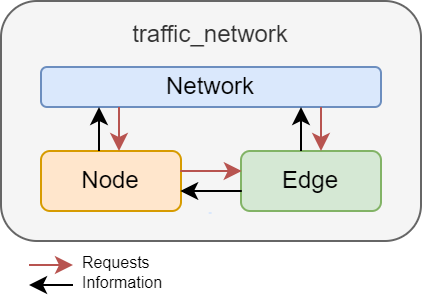
\includegraphics[width=0.5\textwidth]{tex files/Figures/traffic_network_module.png}
	\caption[Network Module:  traffic\_network]{Hierarchical structure of classes within the traffic\_network module.  Directions of requests and information flow between classes is depicted by colored arrows }
	\label{fig:network_module}
\end{figure}


\subsection{Car Module:  network\_cars}

\par "Car" is the general term I use to describe an object traversing the network as it allows for intuitive labeling of its attributes.  Once instantiated, a car is not dependent on the network to continue existing; to represent this semi-independence, the Car class was moved to a separate module:

\begin{figure}[H]
    \centering
	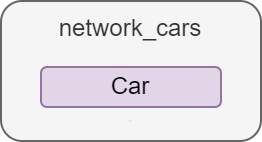
\includegraphics[width=0.3\textwidth]{tex files/Figures/car_module.png}
	\caption[Car Module:  network\_cars]{Classes structure within the network\_cars module}
	\label{fig:cars_module}
\end{figure}

\par In practice, though, the car is not very interesting when trying to simulate overall network behavior and ensuing traffic scenarios.  Any attributes the user may care about (such as current location) are only relevant in context.  So while \textbf{network\_cars} technically exists as a self-contained module, it is never used in isolation.  Instead, this module is automatically imported into the \textbf{traffic\_network} module, seamlessly allowing these two modules to interact with one another.


\subsection{State Module:  Traffic}

\par The final component necessary to creating a simulation  is a mechanism for advancing the state of the network.  State changing includes adding, removing, and advancing any cars on the network as far as possible within a particular unit of time, and are all essential for creating a hands-off simulation. \\

\par But simulation state refers to more than the set of current car locations.  It includes system metadata (like lists of nodes and edges in a network, and their attributes) and dependent calculations from that metadata.  By allowing the user an access point to adapt any component of the network, this software achieves its goal of being adaptable and extensible to other types of networks and simulations.  \\

\par The Traffic modules serves as an API to the underlying simulation, allowing users to (indirectly) interact with the network components and car objects.  The set of all these access points into the simulation allows for the direct management of traffic and has thus been wrapped into an aptly named class,  \textbf{TrafficManager}:

\begin{figure}[H]
    \centering
	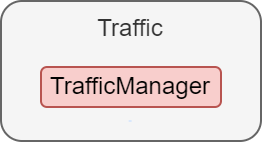
\includegraphics[width=0.3\textwidth]{tex files/Figures/traffic_manager_module.png}
	\caption[State Module:  Traffic\_cars]{Classes structure within the Traffic module}
	\label{fig:traffic_module}
\end{figure}


\noindent  Note that the \textbf{Traffic} module allows only for indirect access to the simulation components.  By using this API as an intermediary between users and network simulation components, the user is given access only to commands that are relevant to analysis, and hide internal functions that facilitate those actions.  For example, if a user wants a particular car to halt in place, they can call on the API function that requests it.  The \textbf{Traffic} module then passes that request to the \textbf{traffic\_network} and/or \textbf{network\_cars} module to handle if and when it becomes relevant.


\section{Essential Module Interaction}

\par Putting the modules together, we get the following depiction of how the modules interact with one another:

\begin{figure}[H]
    \centering
	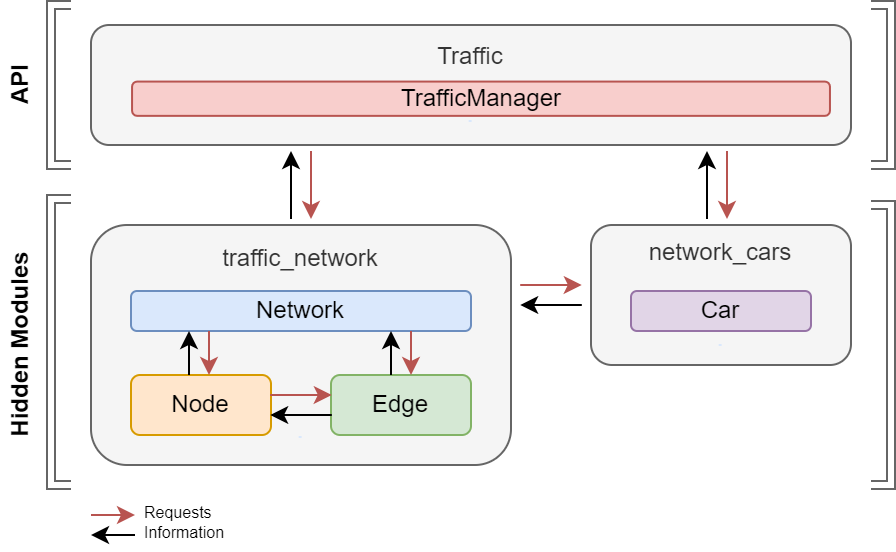
\includegraphics[width=0.9\textwidth]{tex files/Figures/detailed_essentials.png}
	\caption[Software Interaction:  Full View]{Full view of interactions between the modules and their individual components}
	\label{fig:interactions_detailed}
\end{figure}

\noindent  However, as the user doesn't need to concern themselves with the specifics on which functions in which classes work and when, we can streamline the architecture diagram to:

\begin{figure}[H]
    \centering
	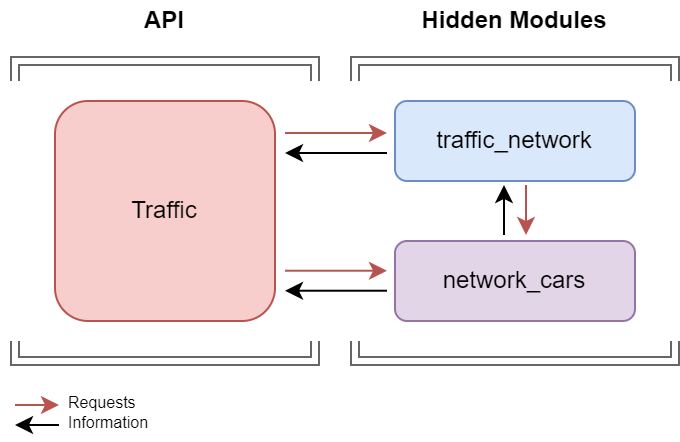
\includegraphics[width=0.7\textwidth]{tex files/Figures/simplified_essentials.png}
	\caption[Software Interaction:  User View]{Generalized overview of interactions between modules}
	\label{fig:interactions_simplified}
\end{figure}



\section{Extended Module Interaction}

Two optional additional modules for generating the underlying network and the car objects themselves can be integrated into the 
% \usetikzlibrary{positioning,matrix,shapes.arrows}

% \tikzset{
%   modulematrix/.style={draw=blue!50!red,rounded corners,matrix of nodes,row sep=1cm,column sep=1cm,nodes={draw=green!70,align=center,font=\sffamily},inner ysep=0.5cm},
%   module/.style={rounded corners, align=center, font=\sffamily, thick},
%   simple module/.style={module, top color=blue!10, bottom color=blue!35, draw=blue!75, text width=40mm, minimum height=15mm},
%   module down arrow/.style={module arrow, shape border rotate=-90},
%   module right arrow/.style={module arrow},
% module arrow/.style={single arrow, single arrow head extend=2.5mm, draw=gray!75, inner color=gray!20, outer color=gray!35, thick, shape border uses incircle, anchor=tail,minimum height=0.7cm},
% }

% \begin{tikzpicture}
% \node [simple module] (mA) {Item-1};
% \matrix[modulematrix,below=of mA,label={[anchor=south]below:Item-2}] (mB) {Item-3 & Item-4 \\};
% \matrix[modulematrix,right=of mB,nodes={text width=5cm,align=center},label={[anchor=north]above:Module C}] (mC) {Item-5 \\ Item-6 \\};
% \matrix[modulematrix,below=of mC,label={[anchor=south]below:Item-9}] (mD) {Item-7 & Item-8 \\};

% \foreach \n in {mA,mC-1-1,mC,mD}
%   \node[module down arrow,below=1mm of \n] {};

% \foreach \n in {mB-1-1,mB,mD-1-1}
%   \node[module right arrow,right=1mm of \n] {};
% \end{tikzpicture}
\chapter{User Manual}
\label{Manual}

\par This chapter illustrates how the traffic simulator software works by guiding the reader through one hypothetical road-traffic simulation step by step in sections 5.1 through 5.5.  Though automotive traffic is used for the example case, instances where the given car simulation may differ from other types of network simulations have been highlighted. \\

\section{Define the scope of the simulation}

\par The details of setting up the simulation depend on several factors:

\begin{enumerate}
    \item What type of network system is being modeled?
    \item What is the goal of the simulation? 
    \item What types of objects traverse the network?  Are the uniform?
    \item What data is already available to create the simulation?  If none, what do we know about the system?
    \item What changes or additions need to be made to a basic network structure to model the idiosyncrasies of the network or desired observations?
    \item How long will the simulation run?  Or how what criteria needs to be met before the simulation is complete?
\end{enumerate}

\noindent For our walkthrough example, the answers might look like the following:

\begin{enumerate}
    \item A province's road network.  Some roads are one-way, and some roads have multiple lanes per direction.
    \item  We want to analyze if adding more highway lanes reduces traffic during rush hour.
    \item Cars and shipping trucks share the road.
    \item There is geospatial data available for city roads (in csv format).  However, there is only one lineitem per named road segment.  We don't have car data, but we know that during the daily rush hour period around 8000 cars travel northbound.
    \item Trucks tend to go 10\% slower than the speed limit.  Everything else seems normal or standard enough. 
    \item We want to observe the simulation for a window of time 1 hour before to 1 hour after rush hour.  We will need to run two simulations (one including the extra highway lanes and one without).
\end{enumerate}


\section{Identify or create the required data}

\par This software requires that network and car objects be imported as a dictionary objects.  At the bare minimum, each imported network requires 2 or more nodes and 1 or more edges (with start and end node IDs specified), with unique identifiers for each.  Each imported car requires (at minimum) a unique identifier and a start and end location for the journey it will take. Users may specify additional attributes that align with their simulation scope, but these are not essential for a simulation to run. \\

\par Users feed information into the simulation by providing specially-formatted objects (json or otherwise).  A complete view of the file format can be found in \autoref{Configs} (Appendix), but the main thing to note is that very few fields are mandatory. \\

\par The Network config file consists of two parts:  Node list and Edge list.  The only mandatory field for Nodes is the \textit{id} as a unique identifier, but users may also add details on stoplights/passage gates (if applicable).  Edges have a few more required attributes (\textit{id}, \textit{start\_node\_id}, \textit{end\_node\_id}), but also allow the user to specify conditions for metering like speed and maximum capacity.  Real-world simulations will typically require the user to specify \textit{edge_length} as well, though the simulation will run regardless, defaulting to equal-length edges (if none specified).


\subsection{Object creation}

\par Users can create the objects themselves, or use the optional \textbf{CarGenerator} and \textbf{UnderlyingNetworkGenerator} modules to output such files. These config files are necessary to launch a new simulation, but are also the expected format of any additions to the network or simulation during the run time.  Any objects imported after initialization should only include new objects.\\

\par Because the simulation has been designed to be capable of importing objects from another simulation's outputs, it should be noted that the config files can be combined into one document.


\subsection{Example}
 \par  Back to our simulation example. \ we identified an existing dataset for network that needed formatting and a schema (but no data) for creating cars.  This requires reformatting the csv network data and using the \textbf{CarGenerator} module (described in a colleague's thesis) to create the cars. \\
 
\par To use the network csv data, we first need rename and reconfigure the fields to match those required to match the our scope, then convert the file from csv to json.  In this case, the steps required are:

\begin{enumerate}
    \item Rename the start and end node fields, and label the edge identifier field as "id". 
    \item Redefine speed.  If the daytime speed limit is 60 km/h but we want our system to have a tick size (process new state) of 1 second to improve simulation accuracy.  Converting to meters per second, that max\_speed is now 16.667.
    \item Create mirror edges for segments labeled "bidirectional".  If edge 1789 is bidirectional and goes from A to B, then we need to create a new edge with a new unique ID that goes from B to A.
    \item Duplicate edges to represent the multiple lanes.  If the highway is currently 4 lanes wide, then 3 additional copies are needed for each edge representing the highway.
    \item Create a second copy of the network file, but add extra edges representing the extra lane on the freeway.
    \item Convert the csv(s) to json.
\end{enumerate}

\noindent If we decided to create cars manually instead, we could use the DEFAULT car config file to to batch out the creation of two car types:  cars (who travel like normal), and trucks (who drive 10\% slower, which translates to setting a default max\_tick\_potential to 0.9).

\section{Set up a new simulation environment and translate the scope to code }

\par The \textbf{Traffic} module serves as an API into the simulation controls; to use \textbf{Traffic} and either of the optional generator modules in the Traffic Network Simulator, the user must import them into their workspace. \\

\par Set up a new python file with the following (or something similar), downloading/installing the modules and (default) config directory associated with this software. \\

\par In your working file, use relevant calls to the \textbf{Traffic} API to build your simulation.  Generally, this includes building a script that calls for a certain amount of ticks, adding cars at relevant points along the way.  For more complex simulations, the user may want to use commands to pause or resume the motion of particular cars (simulating traffic accidents) or prevent access to entire roads/sections of the network.  Please refer to the \autoref{Appendix}, \textit{"\nameref{Appendix}"}, for a full list of API commands available in the current software version. \\

\par For our working rush hour traffic example, we have the following things to consider:

\begin{itemize}
    \item Import the car and (two) network config files and store them as dictionary objects.  Note:  The car objects are assumed to be stored in file after generation here, but that is not necessary.
    \item Since we are running 2 simulations (the existing road network with and without the additional lanes), we need to instantiate one TrafficManager per simulation.
    \item Determine how many ticks the simulation(s) must run for.  If "rush hour" is 2 hours and we want to also capture the hour before and hour after, we need our simulation to run for 4-hours' worth of ticks.  Since the max\_speed precision is defined as meters per second, the simulation should run for 14400 ticks.
    \item Batch out when cars enter the network wince the 8000 cars obviously do not all start driving at the same time.  Perhaps for the first half hour, 400 cars enter, 800 the next half hour, 1500 for the next four half hours, then 400 for the last 2 half hours. (Though there are more accurate ways to model network enter time than these discrete buckets, that choice is left to the user).
    \item Store network snapshots.  One snapshot per tick may be excessive, but a snapshot every minute may be reasonable.  This could translate to grabbing a snapshot every 60 ticks.
\end{itemize}

\noindent To translate these steps to code, we can loop TrafficManager.tick() for as many ticks are needed between snapshot dumps (TrafficManager.get\_snapshot()) and car additions (TrafficManager.add\_car(Car\_ID)).  For an example Simulation working file, refer to \autoref{SampleCode} (Appendix).


\section{Interpret the simulation outputs}

\par When running tm.tick(), a pair of statements will print in the terminal for each tick:

\begin{itemize}
    \item "Steps needed to process tick:  n"
    \item "Percent of available energy used on tick:  m.00\%"
\end{itemize}

\noindent Due to how the tick function works, the full set of nodes and edges will processed as many times as it takes for no more energy to exist or the tick to cause all cars to use up their energy potential. This number of iteration will be 1 if no cars are able to move at all (due to having completed their journey or being labeled temporarily by the user as "immobile"); but more frequently the minimum count is 2 due to a second pass checking if any more motion is possible.  Any number higher than this is a proxy for how complicated the current state change is, but holds no direct meaning on its own. \\

\par However, the second item holds more weight.  Since cars move by using tick potential, if something is preventing a car from moving, movement potential will remain at the end of the turn, indicating that some kind of bottleneck or obstruction is in the way.  Due to the random order of node and tick processing, the user should refrain from taking the energy consumption as a direct metric of congestion, but instead use a moving window average to detect trends or even a global average when comparing simulations (if evaluating the difference a capacity meter, or speed limit change, etc can make). \\

\par  Of course, the user can also elect to save snapshots of the whole network simulation at any point in time.  These snapshots can be individually analyzed for a detailed overview of current network state, or aggregated with a database to observe or compare individual (or categories of) cars and edges.


% \chapter{Use Cases}
\label{Uses}
\chapter{Next Steps}
\label{Future}

\par As this is the first version of the Network Traffic Simulator software, there are several aspects that can be added or improved upon in successive iterations.  Some features are already hinted at in the code itself with placeholder functions, and others don't involve the existing code at all.  This version succeeded in building a functional and extensible traffic simulator that, due do its modularity, can be easily tweaked and expanded by users or future contributors.  Generally, the improvements fall into three categories:  software improvements, feature expansion, and creating a visualizer.

\section{Software Improvement}

\par software design-wise, the system is solid in that its logic is predictable and airtight, and that the system is extensible.  However, there are still many changes that can be made to improve the simulator, particularly in terms of computational complexity.

\begin{enumerate}
    \item \textbf{Subclasses}:  Though the use of subclasses is at odds with the design considerations outlined earlier in the paper, the current use of \textbf{if} statements to check for particular properties is not completely in line with the principle of extensibility.  To remedy this, the use of subclasses should be considered for nodes (stoplights/none) and for cars (static versus dynamic path-following).
    \item \textbf{Tick processing}:  Currently, each tick cycle processes all cars on every single node and edge in the network, and cycles are repeated until no mar cars move.  This means that the edges without cars are checked on each pass, and cars that are immobile or finishes moving for the timestamp are checked with each network tick cycle.  At the cost of increasing memory complexity to store extra variables and statuses, some drastic improvements in computational complexity can be made by doing so.
    \item \textbf{Logs instead of prints}:  While the two status messages printed per tick are beneficial for debugging and analyzing short simulations, they clutter the terminal and bury other print statements (like Exceptions) that may be more important.  The next version will include an option for the user to toggle which kinds of print statements they want to see (car additions, car trip completitions, tick data, etc) and specify a log file to dump them to.
\end{enumerate}


\section{Feature Expansion}

\par Building on the existing framework, the following features can and should be added to future releases:

\begin{enumerate}
    \item \textbf{Remove Node/Edge}:  While the simulator currently supports the addition of nodes and edges into a running simulation, there is only a placeholder for removal so far.  This was due partly in the interest of time, but also due to the question of how cascading effects should be handled:
        \begin{itemize}
            \item If an edge is removed, what happens to the cars that were on that edge or waiting to enter the network along that edge? 
            \item What about if a node is removed?  Should this remove all inbound and outbound edges associated with the node?
            \item Should cars lost in the removal be flagged with the generic "Removed from the simulation at X' status, or would something else provide more insight to the users?
            \item Should removed edges be catalogued like removed cars are?
        \end{itemize}
    Ideally, other users should be surveyed for input before any solution is proposed.
    \item \textbf{Stoplights}:  Currently stoplight change logic is available in the \textbf{traffic\_network} module and it defines the active stoplight setting as the set of edges currently allowing cars to exit.  However, this logic has not yet been activated during the node tick process.  Before adding a check for stoplight presence and status, additional input is requested from users whether the existing stoplight state (at the node level) makes sense at all.
    \item \textbf{Smarter path calculations}:  The current software version includes the option to select the best route based on shortest completion time in normal circumstances, but does not include any option for recalculating around traffic jams/congestion.  This is done somewhat on purpose as a PhD student my supervisor is working with is creating reinforcement learning models that identify these (literal) roadblocks and circumvent them.  Additionally, before a "Fastest\_now" calculation can be created, a more consistent and intuitive metric for congestion levels is needed.
    \item \textbf{Congestion Metric}:  Currently there exists a proxy for network congestion levels (it's the "Percent of available energy used on tick" print statement for each tick call to the \textbf{Traffic} module.  While it would be simple to consider the used energy metric per individual edge, there is not enough evidence (yet) that this is a useful or insightful metric.  We must consider the following:
        \begin{itemize}
            \item Currently congestion is considered in terms of total energy consumption and on the network level.  But would it make more sense to report on the car level (the number of individual cars that were able to move their full distance, the number that were stuck at a complete standstill, and/or the average tick potential used by cars that used some in-between amount)?
            \item Or should congestion be considered as the average of edge-level congestion?
            \item Are we even on the right track associating congestion with movement potential?  Perhaps we should define it in terms of the ability of a new car to enter the network:  What is the available remaining capacity per edge?
        \end{itemize}
\end{enumerate}


\section{Visualization}

\par Currently, the only way a user can view the output of a simulation is by saving and viewing snapshots.  These snapshots were explicitly designed to be used for generating a simulation visualization, but the visualizer itself was not yet created due to time constraints.  Below is a proposal for building a visualizer:

\begin{itemize}
    \item \textbf{Simulation precision}:  As the simulation runs in discrete tick intervals, it makes sense to update the visualization with each tick, which can be done by utilizing the "get\_snapshot" function already created for this purpose.  While this does not create a continuous simulation, true continuity is not achievable due to the code design.  However, continuity can be approximated by using animations to transition the image from one tick state to the next.
    \item \textbf{Snapshot deltas}:  In the current version of the code, you can find a placeholder function labeled "get\_snapshot\_deltas", which would report only the \textit{differences} between one snapshot and the next (rather than dump data for the entire network).  Creating this function would allow a much smaller file to be sent to whatever server would host the visualizer, though is entirely non-essential for local instances or small simulations.
    \item \textbf{Implementation}:  Because the visualizer will be built from the snapshot json files, the language that the visualizer is written in doesn't need to match the simulator.  Instead, we can use JavaScript to take advantage of the \textbf{vis.js} library or \textbf{D3.js} library, each specifically written to display (dynamic) graphs.
        \begin{itemize}
            \item vis.js provides simple graphs off the bat.  While it doesn't seem like it (easily) supports the ability to add objects (cars) to the edges, you can change the displayed elements to reflect attributes weights.  This would allow you to create a visualization displaying congestion, where the thinkness of the edge between two nodes is proportional to congestion.  This can be beneficial for visually isolating traffic bottlenecks. D3.js appears very much the same.
            \item Another option for simulations based on real-world geographic data is to utilize the ArcGIS API.  While this does not solve the issue of displaying cars on the network, it does accurately reflect the relative relations and distances between and two nodes, whether they are connected or not.
        \end{itemize}
\end{itemize}
\chapter{Appendix}
\label{Appendix}

\par This sections contains excerpts from the Network Traffic Simulator code and an overview of the system this software was created and tested on.  The version you see here is the complete documentation for version 1.0.0, released  1 July 2022.  \\

\noindent The features found in this version were created to meet (and exceed) the requirements and expectations set  by Universiteit Utrecht staff and serves as a graduation thesis project for their MSc Applied Data Science program.  This release, while a bit barebones on the generator side, sets up a complete, adaptable framework for urban traffic simulations (and other use cases!). \\

\noindent Please check the repository below for the latest instantiation:
\begin{verbatim}
    https://github.com/julialruiter/Traffic_Simulator
\end{verbatim} 

%%%%%%%%%%%%%%%%%%%%%%%%%%%%%%%%%%%%%%%%%%%%%%%%%%%%%%%%%%%%%%%%%
%---------------------------------------------------------------%
\section{Dependencies}
So much as possible, libraries have been kept to the standard Python libraries.  This means that the current Network Traffic Simulator software version has no external dependencies.

%%%%%%%%%%%%%%%%%%%%%%%%%%%%%%%%%%%%%%%%%%%%%%%%%%%%%%%%%%%%%%%%%
%---------------------------------------------------------------%
\section{System Specifications}
This software was created and tested on a machine with the following specifications.  Though no official stress-testing has been done for this publication, this information may be relevant in analyzing any metrics reported in follow ups: \\

\begin{center}
    \noindent \begin{tabular}{l l}  %{>{\bfseries}l p{6cm}}
    \toprule
    \textbf{OS Name} & Microsoft Windows 10 Home\\
    \midrule
    \textbf{OS Version} & 10.0.19044 N/A Build 19044\\
    \midrule
    \textbf{OS Configuration} & Standalone Workstation\\
    \midrule
    \textbf{OS Build Type} & Multiprocessor Free\\
    \midrule
    \textbf{OS Build Type} & Multiprocessor Free\\
    \midrule
    \textbf{System Manufacturer} & ASUSTeK COMPUTER INC.\\
    \midrule
    \textbf{System Model} & VivoBook\_ASUSLaptop X521EA\_S533EA\\
    \midrule
    \textbf{System Type} &  x64-based PC\\
    \midrule
    \textbf{Processor} & Intel64 Family 6 Model 140 \\
    & Stepping 1 GenuineIntel ~2803 Mhz \\
    \midrule
    \textbf{Installed RAM} & 16.0 GB (15.7 GB usable)\\
    \bottomrule
    \end{tabular}
\end{center}
 \\
 
%%%%%%%%%%%%%%%%%%%%%%%%%%%%%%%%%%%%%%%%%%%%%%%%%%%%%%%%%%%%%%%%%
%---------------------------------------------------------------%
\section{API Module: Traffic.py}
This module instantiates a simulation instance and exposes all necessary/desired functions for interacting with the simulation once it is running:

\subsection{class TrafficManager:}

\begin{alltt}
\textbf{__init__}(self, network_config) -> None
Establishes an instance of TrafficManager to run on the given 
network structure.
Attributes:
    graph:  Network object that the TrafficManager runs on.
    timestamp:  Simulation timestamp.

\textbf{add_car}(self, car)
API function:  place car (dictionary object) onto the network's 
waiting queue.
Please note that the current iteration of add_car only supports 
placement directly onto Edges (identified by "start_edge").

\textbf{get_all_paths_A_to_B}(self, start_edge_ID, end_edge_ID)
API function:  Given a start and end Edge id, return a list of 
all valid paths that do not repeat Edges.

\textbf{get_node_edges_in_out}(self, node_ID)
API function:  lists the IDs of inbound and outbound edges for 
a particular node.
This information can also be found via 'get_snapshot()'.

\textbf{get_path_distance}(self, path)
API function:  Given the ordered list of Edges as "path", 
evaluate the total distance it would take to travel.
This function assumes that the entirety of each Edge is 
traveled.

\textbf{get_path_minimum_time}(self, path)
API function:  Given the ordered list of Edges as "path", 
evaluate the minimum time it would take to travel (in ticks) 
given each Edge's speed limit.
Minimum time is calculated assuming a car is able to travel 
the maximum speed per edge unencumbered.
This function assumes that the entirety of each Edge is 
traveled and includes any Node-crossing time penalties.
\textit{Note:  time cost does NOT include Node-crossing time out of the 
final edge as the Car is expected to exit the Network before the 
Edge's end.}

\textbf{get_shortest_path_A_to_B}(self, all_paths_list)
API function:  Given all_paths_list (a list of paths from A to 
B as calculated using self.get_all_paths_A_to_B()),
returns the path with the shortest total distance in terms of 
length.

\textbf{get_snapshot}(self)
API function:  outputs list of nodes, edge attributes, car 
attributes.
Output is formatted in such a way that it can be used as input 
for a new simulation.

\textbf{get_theoretical_fastest_path_A_to_B}(self, all_paths_list)
API function:  Given all_paths_list (a list of paths from A to 
B as calculated using self.get_all_paths_A_to_B()),
returns the path with the minimum total travel time (assuming no
congestion).

\textbf{get_timestamp}(self)
API function:  returns (sequential) state number.

\textbf{pause_car}(self, car_id)
API function:  forcefully halts the Car associated with 'car_id' 
until a 'resume_car' call is received.
No cars behind it may pass.

\textbf{remove_car}(self, car_id)
API function:  removes the Car associated with 'car_id' from
the simulation.
This is done by forcing it into Car.status = 'Removed from 
simulation'.

\textbf{resume_car}(self, car_id)
API function:  allows the Car associated with 'car_id' to 
resume moving.

\textbf{tick}(self)
API function:  advance state of network by one unit of time.


\end{alltt}

%%%%%%%%%%%%%%%%%%%%%%%%%%%%%%%%%%%%%%%%%%%%%%%%%%%%%%%%%%%%%%%%%
%---------------------------------------------------------------%
\section{Hidden Module: traffic\_network.py}

This module creates and runs an instance of a Network object when a simulation is created via starting a \textbf{TrafficManager} instance.  The main item here is \textbf{class Network}, which  contains, creates, and collects several dependent components (\textbf{class Node}, \textbf{class Edge}, and \textbf{class Car}).  \\

\noindent The functions here should be hidden from the user.  Instead, the user should call for changes using the\textbf{TrafficManager} API.  Internal functions belonging to the \textbf{traffic\_network} module can be seen below:

%%%%%%%%%%%%%%%%%%%%%%%%%%%%%%%%%%%%%%%%%%%%%%%%%%%%%%%%%%%%%%%%%
%---------------------------------------------------------------%
\subsection{class Network:}

\begin{alltt}
\textbf{__init__}(self, TrafficManagerPointer, config) -> None
Contains all functions and attributes pertaining to the (road) 
network as a whole.
Attributes:
    \textbf{TrafficManager_pointer}:  Identifies which TrafficManger 
    simulation is associated with this network
    \textbf{node_ID_to_node}:  Dictionary mapping Node IDs to Node objects.
    \textbf{edge_ID_to_edge}:  Dictionary mapping Edge IDs to Edge objects.
    \textbf{car_ID_to_car}:  Dictionary mapping Car IDs to Car objects.
    \textbf{global_tick}:  Tick index, aligns with TrafficManager tick

\textbf{add_car}(self, car)
Places Car (object) on the waiting queue for its specified 
start_edge.
Validity checks have been passed up to the TrafficManager level 
as a part of "add_car(car)",
ensuring that any Cars received are valid OR can be made valid 
using the DEFAULT_car_values_config.json file.

\textbf{add_edge}(self, edge)
Imports edge(s) from given edge dictionary.
If both the start and end nodes are already in the network, then 
the edge will be added.
Any Edge attribute values not given in the edge object (imported) 
will instead be assigned from the imported defaults file:
edge_default_config.
\textit{Note:  there are no default values for id, start_node_id, nor 
end_node_id as these are an Edge's unique identifiers.}

\textbf{add_node}(self, node)
Imports node(s) from given node dictionary and adds them to 
the network.

\textbf{all_paths_depth_first_search}(self, current_edge_ID, 
end_edge_ID, visited_list=[], valid_paths=[])
Given a start and end Edge id, return a list of all valid paths 
that do not repeat Edges.

\textbf{check_valid_car}(self, car)
Returns a detailed Exception if the given car does not conform 
to expected input structure.

\textbf{choose_path}(self, all_paths_list, metric)
Given a list of paths from A to B (ex: as calculated using
self.all_paths_depth_first_search()),
returns the "best" path with regards to input metric.
Currently supported input metrics:
    \textbf{'Fastest'}: best path = minimum total travel time (assuming 
    no congestion).
    \textbf{'Shortest'}: best path = shortest total distance in terms of 
    length.
    \textbf{'Random'}:  pay no heed to metics, choose an available path 
    at random.
Future versions may include metrics like:
    \textbf{'Fastest_now'}: best path = minimum travel time after 
    accounting for current Network congestion.

\textbf{get_Network_pointer}(self)
Returns tick index (which aligns with TrafficManager tick).

\textbf{get_edge_id}(self, edge_id)
Uses Network.edge_ID_to_edge dictionary to map an Edge ID to 
its corresponding Edge object.

\textbf{get_global_tick}(self)
Returns a pointer to this Network instance.
Useful for directly generating cars OR keeping track managing 
multiple simulations at once.

\textbf{get_node_from_id}(self, node_id)
Uses Network.node_ID_to_node dictionary to map a Node IDs to 
its corresponding Node object.

\textbf{get_snapshot}(self)
Outputs dictionary containing snapshot data for all nodes and 
edges in the network.

\textbf{path_cost_distance}(self, path_list)
Given path_list, evaluate the total distance it would take to 
travel.
This function assumes that the entirety of each Edge is traveled.

\textbf{path_cost_minimum_time}(self, path_list)
Given path_list, evaluate the the minimum time it would take to 
travel (in ticks) given each Edge's max_speed.
Minimum time is calculated assuming a car is able to travel the 
maximum speed per edge unencumbered.
This function assumes that the entirety of each Edge is traveled 
and includes any Node-crossing time penalties.
\textit{Note:  time cost does NOT include Node-crossing time out of the 
final edge as the Car is expected to exit the Network before the 
Edge's end.}

\textbf{remove_edge}(self, edge)
Placeholder for future software version:
Will remove an Edge and all of its associated Cars from the 
Network.

\textbf{remove_node}(self, node)
Placeholder for future software version:
Will remove a Node and all of its associated inbound/outbound 
Edges from the Network.

\textbf{restore_tick_potential}(self)
Resets the tick_potential to its maximum value for all Cars on 
the Network.

\textbf{tick}(self)
Shuffles the order in which Node ticks will be processed with 
each global tick to ensure no node is favored.
\textit{Note:  global tick != Node tick.  Global tick is the unit of 
time until the next state of the simulation, 
while Node tick the proportion of that time that its components 
can move uninterrupted.  
Node ticks will occur until the sum of their durations reaches 
that of a global tick/no further movement is possible.}

\end{alltt}


%%%%%%%%%%%%%%%%%%%%%%%%%%%%%%%%%%%%%%%%%%%%%%%%%%%%%%%%%%%%%%%%%
%---------------------------------------------------------------%
\subsection{class Node:}

\begin{alltt}
\textbf{__init__}(self, Network_reference, id, intersection_cost,
stoplight_pattern, stoplight_duration, stoplight_delay) -> None
Contains all functions and attributes pertaining to a network 
intersection (Node).
Attributes:
    \textbf{id}:  Unique ID associated with this Node object.
    \textbf{inbound_edge_ID_to_edge}:  Dictionary mapping inbound Edge 
    IDs to Edge objects.
    \textbf{outbound_edge_ID_to_edge}:  Dictionary mapping outbound Edge 
    IDs to Edge objects.
    \textbf{intersection_time_cost}:  Value representing time in ticks 
    required to cross intersection.  0 <= value < 1.
    \textbf{stoplight_pattern}:  Ordered list of sets of simeltaneous 
    Edges eligible for car exiting. Pattern cycles through sets. 
    (Will be implemented in future versions of the software).
    \textbf{stoplight_pattern_current_index}:  Index representing which 
    set of stoplight_pattern the Node is currently on.  (Will be
    implemented in future versions of the software).
    \textbf{stoplight_duration}: Number of ticks that the stoplight_pattern 
    stays on its current Edge set. (Will be implemented in future 
    versions of the software).
    \textbf{stoplight_delay}: Number of ticks between change of 
    stoplight_pattern Edge sets. (Will be implemented in future 
    versions of the software).
    \textbf{node_tick_number}:  Used in stoplight changes, increments by 
    one with each global TrafficManager tick. 

\textbf{add_to_inbound}(self, edge)
Used when adding an Edge to the Network when 
Edge.end_node == self.id .
Adds the Edge ID and a mapping to its corresponding Edge object 
to the inbound_edge_ID_to_edge dictionary.

\textbf{add_to_outbound}(self, edge)
Used when adding an Edge to the Network when 
Edge.start_node == self.id .
Adds the Edge ID and a mapping to its corresponding Edge object 
to the outbound_edge_ID_to_edge dictionary.

\textbf{get_inbound_exit_candidates}(self)
Checks all inbound edges of a Node.  
Any edge that has a Car at the end position of its length is 
considered a candidate to advance on to the next Edge in its 
path.

\textbf{get_intersection_time_cost}(self)
Returns self.intersection_time_cost, the time penalty it takes 
to cross a Node.
\textit{Note:  this value may be 0.}

\textbf{get_node_ID}(self)
Returns self.id.
Used when calling value from outside the Node class.

\textbf{get_node_inbound}(self)
Returns the keys to the dictionary self.inbound_edge_ID_to_edge, 
list of all inbound Edge IDs.
Used when calling from outside the Node class.

\textbf{get_node_outbound}(self)
Returns the keys to the dictionary self.outbound_edge_ID_to_edge, 
list of all outbound Edge IDs.
Used when calling from outside the Node class.

\textbf{get_snapshot}(self)
Outputs dictionary of Node attributes.

\textbf{tick}(self)
Facilitates Edge ticks and movement of Car objects from one Edge 
to another.
If a Car that is eligible to cross the Node has type "Dynamic", 
then its path is recalculated upon crossing.
Each Node tick shuffles the order in which Edges tick to ensure 
no particular Edge is favored.

\textbf{update_stoplight_attributes}(self)
Toggles which Edges allow cars to exit by cycling through sets 
in stoplight_pattern.
Returns the set of which inbound Edge set in stoplight_pattern is
currently active, or NULL set (denoting red lights for all edges).
Communication to TrafficManager to establish global tick and 
increment will be solved in future versions.
Communication to prevent cars from leaving inbound Edges during 
the node tick will be established in future versions.

\end{alltt}

%%%%%%%%%%%%%%%%%%%%%%%%%%%%%%%%%%%%%%%%%%%%%%%%%%%%%%%%%%%%%%%%%
%---------------------------------------------------------------%
\subsection{class Edge:}

\begin{alltt}
\textbf{__init__}(self, id, start_node_id, end_node_id, edge_length,
max_speed, max_capacity) -> None
Contains all functions and attributes pertaining to a road 
segment (Edge).
Attributes:
    \textbf{id}:  Unique ID associated with this Edge object.
    \textbf{start_node_id}:  Node from which this Edge originates (this
    Edge is an outbound_edge for start_node).
    \textbf{end_node_id}:  Node from which this Edge terminates (this 
    Edge is an inbound_edge for end_node).
    \textbf{start_node}:  Node object represented by start_node_id.
    \textbf{end_node}:  Node object represented by end_node_id.
    \textbf{edge_length}:  Physical length of the Edge (ex: meter length
    of a road).  Default value can be found and adjusted at
    edge_default_config["edge_length"]
    \textbf{max_speed}:  (optional) Unit speed limit of the road.  
    Without obstructions, this is the maximum distance a Car 
    can move on this Edge in one tick.  Default value can be 
    found and adjusted at edge_default_config["max_speed"]
    \textbf{max_capacity}:  (optional) Maximum number of Car objects
    allowed on the Edge (max length of current_cars). Default 
    value can be found and adjusted at 
    edge_default_config["max_capacity"]
    \textbf{edge_car_ID_to_car}:  Dictionary containing all Car objects
    associated with the Edge; maps Car IDs to Car objects.
    \textbf{current_cars}:  List of IDs of all Cars currently on the Edge.
    \textbf{waiting_cars}:  List of IDs for Cars that are trying to enter
    the Network at this Edge.
    \textbf{processed_cars}:  List capturing IDs of Cars that have already
    been processed on the current tick.  Becomes current_cars at 
    the end of the Edge tick.
    \textbf{completed_cars}:  List of IDs of any Cars that have completed
    their route on this Edge in the duration of the simulation.
\textit{Note:  some attributes have been given default values in the case
that the user did not provide them.}

\textbf{add_car_to_wait_queue}(self, car)
Adds Car object to the waiting queue and links Car to Edge on Car 
ID.

\textbf{get_current_cars}(self)
Returns self.current_cars, the list of Car IDs for all cars 
currently on the Edge.
Used when calling value from outside the Edge class.

\textbf{get_edge_ID}(self)
Returns self.id.
Used when calling value from outside the Edge class.

\textbf{get_end_node}(self)
Returns self.end_node Object.
Used when calling value from outside the Edge class.

\textbf{get_end_node_id}(self)
Returns self.end_node_id.
Used when calling value from outside the Edge class.

\textbf{get_length}(self)
Returns self.edge_length (length of road segment, typically in 
meters).
Used when calling value from outside the Edge class.

\textbf{get_max_capacity}(self)
Returns self.max_capacity.
Used when calling value from outside the Edge class.

\textbf{get_max_speed}(self)
Returns self.max_speed (speed limit of road segment, typically
in meters/sec).
Used when calling value from outside the Edge class.

\textbf{get_snapshot}(self)
Outputs dictionary of Edge attributes, including lists of Cars 
that are:  currently on the Edge, waiting to enter the Edge, or 
completed their trip on this Edge.

\textbf{get_start_node}(self)
Returns self.start_node Object.
Used when calling value from outside the Edge class.

\textbf{get_start_node_id}(self)
Returns self.start_node_id.
Used when calling value from outside the Edge class.

\textbf{move_existing_car_to_edge}(self, car)
Adds Car object to the 'processed-cars' list and links Car to 
(new) Edge on Car ID.

\textbf{set_current_cars}(self, new_list)
Replaces the list contents of self.current_cars with new_list.
Used when updating value from outside the Edge class.

\textbf{set_end_node}(self, node_ptr)
Associates (end) Node pointer with Edge object.
Used when adding an Edge to the Network.

\textbf{set_start_node}(self, node_ptr)
Associates (start) Node pointer with Edge object.
Used when adding an Edge to the Network.

\textbf{tick}(self)
Facilitates the movement of Car objects traversing this Edge.  
There are three types of movement:
\textbf{car entry}:  a Car from the waiting_car list will be placed on 
the Edge if and when space becomes available.
\textbf{car exiting}:  a Car will exit the Network if and when it reaches
its end_pos_meter in the process of its movement IF 
self.id = Car.end_edge.
\textbf{car movement}:  a Car with status mobile = True will advance as
far as possible (maximum potential distance, edge end, or until 
obstructed by another car).

\end{alltt}



%%%%%%%%%%%%%%%%%%%%%%%%%%%%%%%%%%%%%%%%%%%%%%%%%%%%%%%%%%%%%%%%%
%---------------------------------------------------------------%
\subsection{class Car:}

\begin{alltt}
\textbf{__init__}(self, car_ID, car_length, start_edge, start_pos_meter,
end_edge, end_pos_meter, path, car_type, route_preference,
max_tick_potential) -> None
Contains all functions and attributes pertaining to an object 
traversing the Network (Car).
Attributes:
    \textbf{id}:  Unique ID associated with this Car object.
    \textbf{car_length}:  Physical unit length of the Car object 
    (ex: meters).  May be 0.
    \textbf{start_edge}:  Edge from which this Car originates 
    its journey.
    \textbf{start_pos_meter}:  Unit position along start_edge 
    from which the Car begins its journey.  
    Edge origin = position 0.
    \textbf{end_edge}:  Edge from which this Car terminates its 
    journey.
    \textbf{end_pos_meter}:  Unit position along end_edge at 
    which the Car terminates its journey and leaves the Network.
    \textbf{path}:  Ordered list of Edges that the Car will 
    traverse to get from start to end.
    \textbf{route_preference}:  Classification determining 
    which type of path will be followed:
        if \textbf{'Fastest'}: chooses path with minimum total 
        travel time (assuming no congestion).
        if \textbf{'Shortest'}: chooses path with shortest total 
        distance in terms of length.
        if \textbf{'Random'}:  pays no heed to metrics and 
        instead chooses an available path at random.
    \textbf{car_type}:  Car classification for path-following:
        if \textbf{'Static'}:  Car follows predetermined path 
        set on addition.
        if \textbf{'Dynamic'}:  Car will recalculate its route 
        every time it reaches a Node. 
    \textbf{mobile}:  Car classification for mobility:
        if \textbf{True}:  Car is eligible to move (default).
        if \textbf{False}:  Car has been halted and will not move 
        until further instructions given.
    \textbf{route_status}:  string explaining the Car's status 
    with regards to path completion:
        \textbf{'In progress'}:  The Car is eligible for movement; 
        the Car is moving along its path.
        \textbf{'Route Completed'}:  The Car has reached its 
        destination and has been removed from the Network.
        \textbf{'Paused'}:  The Car is ineligible for movement 
        due to mobile=False.
        \textbf{'Removed from simulation at tick #n'}:  The Car 
        was removed from the simulation by external intervention.  
        n denotes timestamp at which it was removed.
    \textbf{current_edge}:  Edge ID corresponding to the Car's 
    current location.
    \textbf{current_pos_meter_car_front}:  Unit distance along
    current_edge corresponding to the Car's current location.  
    If car_length > 0, this refers to the position of the front 
    of the Car.
    \textbf{max_tick_potential}:  Proportion of global maximum 
    tick time-distance that the Car is eligible to move 
    (default = 1, full potential).
    \textbf{current_tick_potential}:  Portion of tick 
    time-distance that the car has not (yet) utilized on this 
    tick.

\textbf{get_car_ID}(self)
Returns self.id.
Used when calling value from outside the Car class.

\textbf{get_car_length}(self)
Returns self.car_length.
Used when calling value from outside the Car class.

\textbf{get_car_type}(self)
Returns self.car_type.
Value is \textbf{"Static"} (Car remains on its original path) or \textbf{"Dynamic"}
(Car recalculates path at every Node crossing).
Used when calling value from outside the Car class.

\textbf{get_current_edge}(self)
Returns self.car_length.
Used when calling value from outside the Car class.

\textbf{get_current_pos_meter_car_front}(self)
Returns self.current_pos_meter_car_front.
Used when calling value from outside the Car class.

\textbf{get_current_tick_potential}(self)
Returns self.current_tick_potential.
Used when calling value from outside the Car class.

\textbf{get_end_edge}(self)
Returns self.end_edge, the Edge at which the Car finishes its 
route and leaves the Network.
Used when calling value from outside the Car class.

\textbf{get_end_pos_meter}(self)
Returns self.end_pos_meter, the position on the Edge at which 
the Car finishes its route and leaves the Network.
Used when calling value from outside the Car class.

\textbf{get_max_tick_potential}(self)
Returns self.max_tick_potential.
Used when calling value from outside the Car class.

\textbf{get_mobility}(self)
Returns self.mobile.
Value is \textbf{True} (Car is eligible to move) or \textbf{False} 
(Car is halted or its path is complete).
Used when calling value from outside the Car class.

\textbf{get_path}(self)
Returns self.path, the ordered list of upcoming Edges the Car
will traverse.
Used when calling value from outside the Car class.

\textbf{get_route_metric}(self)
Returns self.route_preference.  Used when a Car's path needs 
to be (re)calculated.
Value is "Shortest", "Fastest", "Random", with "Random" being 
the default value if none specified.
Used when calling value from outside the Car class.

\textbf{get_route_status}(self)
Returns self.route_status.
Value is "In progress", "Route Completed", "Paused", or 
"Removed from simulation at tick #n".
Used when calling value from outside the Car class.

\textbf{get_snapshot}(self)
Outputs dictionary of Car attributes.

\textbf{get_start_edge}(self)
Returns self.start_edge, the Edge at which the Car entered 
the Network.
Used when calling value from outside the Car class.

\textbf{get_start_pos_meter}(self)
Returns self.start_pos_meter, the position on the start Edge 
at which the Car entered the Network.
Used when calling value from outside the Car class.

\textbf{set_current_edge}(self, edge_ID)
Replaces self.current_edge with edge_ID.
Used when updating value from outside the Car class.

\textbf{set_current_pos_meter_car_front}(self, new_position_meters)
Replaces self.current_pos_meter_car_front with 
new_position_meters.
Used when updating value from outside the Car class.

\textbf{set_current_tick_potential}(self, new_potential)
Replaces self.current_tick_potential with new_potential.
Used when updating value from outside the Car class.

\textbf{set_mobility}(self, Boolean)
Updates the Boolean value of self.mobile to input Boolean.
Value is \textbf{True} (Car is eligible to move) or \textbf{False}
(Car is halted or its path is complete).
Used when updating value from outside the Car class.

\textbf{set_path}(self, new_path_list)
Replaces self.path with new_path_list, 
typically removing the first entry as the car enters a new Edge, 
or when calculating a new route.
Used when updating value from outside the Car class.

\textbf{set_route_status}(self, new_string)
Updates self.route_status to new_string.
Value should be "In progress", "Route Completed", "Paused", or 
"Removed from simulation at tick #n".
Used when updating value from outside the Car class.

\textbf{tick}(self, old_potential)
Calculates "potential" differential;
This is the portion of a full tick movement completed by the 
Car on this tick.

\end{alltt}


%%%%%%%%%%%%%%%%%%%%%%%%%%%%%%%%%%%%%%%%%%%%%%%%%%%%%%%%%%%%%%%%%
%---------------------------------------------------------------%
\section{Optional Module:  \\ UnderlyingNetworkGenerator.py}
In the absence of a pre-made graph to run the simulation on, the user can elect to use this module to generate a network.  This method of Netowrk generation may be useful for some particular use cases where it is beneficial to create a graph with many Nodes and Edges sharing the same properties.\\

\noindent The current version of this module supports the creation of Erdős-Renyi random graphs OR complete, bidirectional graphs.  This module will be improved later to support other mathematical network types.

\subsection{class NetworkGenerator:}

\begin{alltt}
\textbf{__init__}(self) -> None
Class containing various functions for generation Network objects 
for the simulation to run on.
A Network can also be provided via custom JSON file instead.

\textbf{create_ER_network_default_values}(self, number_nodes,
probability_joining=0.5)
Creates an Erdos Renyi Network based on the given parameters:
A each pair of nodes has a probability_joining (0 < p < 1) of 
being connected in an ER Network.
As this is a directional Network, each pair will be considered 
separately per direction.
This Network uses the following default values:
    probability_joining = 0.5     # can be overwritten by input
    node.intersection_time_cost = 0
Please note that this NetworkGenerator function only generates 
the barebone structures necessary for a Network. 
All additional attributes will be loaded via
"DEFAULT_edge_values_config.json" during the simulation process.

\textbf{generate_complete_bidirectional_network_default_values}(self,
number_nodes)
Generates a complete Network consisting of number_nodes Nodes, 
each connected to every other Node in both directions.
This Network uses the following default value:
    node.intersection_time_cost = 0
Please note that this NetworkGenerator function only generates 
the barebone structures necessary for a Network. 
All additional attributes will be loaded via
"DEFAULT_edge_values_config.json" during the simulation process.
output_Network_dictionary(self, node_dict, edge_dict)
Returns dictionary containing all Node and Edge information for 
the newly generated Network.

\end{alltt}

%%%%%%%%%%%%%%%%%%%%%%%%%%%%%%%%%%%%%%%%%%%%%%%%%%%%%%%%%%%%%%%%%
%---------------------------------------------------------------%
\subsection{class GeneratorNode:}

\begin{alltt}
\textbf{__init__}(self, id) -> None
Contains all attributes necessary for creating a network 
intersection (Node).
Attributes:
    id:  Unique ID associated with this Node object.
    intersection_time_cost:  Value representing time in ticks 
    required to cross intersection.  0 <= value < 1.
\end{alltt}


%-----------------------------------------------------------------%
\subsection{class GeneratorEdge:}

\begin{alltt}
\textbf{__init__}(self, id, start_node_id, end_node_id, edge_length=None,
max_speed=None, max_capacity=None) -> None
Contains all attributes necessary for creating a road segment 
(Edge).
Attributes generated in all NetworkGenerator functions:
    \textbf{id}:  Unique ID associated with this Edge object.
    \textbf{start_node_id}:  Node from which this Edge originates.
    \textbf{end_node_id}:  Node from which this Edge terminates.
Attributes generated only in probabilistic NetworkGenerator 
functions:
    \textbf{edge_length}:  Physical length of the Edge (ex: meter length 
    of a road).
    \textbf{max_speed}:  (optional) Unit speed limit of the road.  
    Without obstructions, this is the maximum distance a Car 
    can move on this Edge in one tick.
    \textbf{max_capacity}:  (optional) Maximum number of Car objects
    allowed on the Edge.
\end{alltt}

%\end{comment}


%%% End of the main matter.
\backmatter

%%%% BIBLIOGRAPHY (Be sure cto compile with BibTeX to make this work!)
%
\nocite{*} % Show everything in bib file, not just things that are explicitly cited.
\bibliography{bibliography}
\bibliographystyle{alpha}


%\printbibliography


\end{document}

% double check/cross with original doc--might be undoing what is going on in 
% have to bibtex bibliography first, then can tex rest of file